\documentclass[a4paper,14pt]{extarticle}
\usepackage[left=2.5cm, right=1.5cm, vmargin=2.5cm]{geometry}
\usepackage[utf8]{inputenc}
\usepackage[T2A]{fontenc}
\usepackage[russian]{babel}
\usepackage{graphicx}
\graphicspath{{pictures/}}
\usepackage{caption}
\usepackage{subcaption}
\usepackage{indentfirst}
\setlength\parindent{5ex}
\usepackage{fancyhdr}
\usepackage{booktabs}
\usepackage{siunitx} 
\usepackage{pgfplotstable}
\usepackage{amsmath}
\usepackage{autonum}
\usepackage{amsfonts}
\DeclareMathOperator{\sign}{sgn}
\newcommand{\gt}{\textgreater} % знак больше
\newcommand{\lt}{\textless}       % знак меньше
\DeclareGraphicsExtensions{.pdf,.png,.jpg}
\pagestyle{fancy}
\fancyhf{}
\rhead{\thepage}
\renewcommand{\headrulewidth}{0pt}

\fancypagestyle{plain}{ 
	\fancyhf{}
	\rhead{\thepage}}

\author{Никитин Илья}

\title{Отчет по лабораторной работе №1: "Основы вакуумной техники"}
\date{\today}

\begin{document}
	
	\maketitle
	\tableofcontents

	\section{Задачи}
		Познакомиться с работой вакуумного оборудования, методами измерения и контроля вакуума.
	\section{Оборудование}
		\begin{itemize}
			\item Arduino Uno
			\item Манометр Pfeiffer TPR281
			\item Вакууметр Мерадат-ВИТ
			\item Термопарный и ионизационный манометрические преобразователи ПМТ-2	ПМИ-2
			\item Манометр Thyracont
			\item Ёмкостный датчик Thyracont
			\item Откачной пост Pfeiffer Vacuum HiCube 80 Eco 
			\item Вакуумная арматура
		\end{itemize}
	\section{Теория}
		Обычно выделяют несколько диапазонов давления, отличающихся режимами молекулярно-кинетических явлений в вакуумной системе:
		\begin{itemize}
			\item Низкий вакуум $1000$ -- $1$ мбар
			\item Средний вакуум $1$ -- $10^{-3}$ мбар
			\item Высокий вакуум $10^{-3}$ -- $10^{-7}$ мбар
			\item Ультравысокий вакуум $10^{-7}$ -- $10^{-14}$ мбар
		\end{itemize}
			\subsection{Линии откачки}
			Важнейшей характеристикой линии откачки является ее пропускная способность, которая определяется так:
			\begin{equation}
				C = \frac{q_{p V}}{\Delta p},
			\end{equation}
			где $q_{p V}$ -- поток газа через линию в единицах $p V$, а $\Delta p$ -- разность давлений на ее концах.
			В вязком режиме для линии круглого сечения длиной $l$ проводимость равна $C = \pi r^4 (p_1 + p_2) / (16 \eta l)$, где $\eta$ - вязкость газа.
			
			Важнейшей характеристикой насоса является его быстрота действия, которая определяется как объем газа, проходящий в единицу времени через входной патрубок насоса:
			\begin{equation}
				|S| = \frac{dV}{dt}
			\end{equation}
			Из предположения, что $\frac{dN}{dt} \sim S p$, получим, что:
			\begin{equation}
				S p = \frac{d p V}{dt} = V \frac{dp}{dt}
			\end{equation}
			То есть:
			\begin{equation}
				S = \frac{V}{p} \frac{dp}{dt}
			\end{equation}
	\section{Описание установки}
		В экспериментах использовался откачной пост, на который с помощью вакуумной арматуры присоединялось всё необходимое оборудование. Достаточно низкие давления (порядка 1 Па и ниже), измеряемые с помощью манометрических преобразователей снимались на вакууметре, а давления порядка 1 Па - $10^5$ Па измерялось на манометре Pfeiffer TPR281 и оцифровывалось с помощью датчика Arduino, кроме того, в одном эксперименте был использован манометр Thyracont, который в первую минуту эксперимента (пока давление не снизилось достаточно, чтобы лампы заработали) снимался на камеру, а затем был отключен, данные с него так же были вручную оцифрованы.
	\section{Предельное давление и скорость откачки}
		\subsection{Ход работы}
			Для того чтобы измерить необходимые параметры, мы подключили к насосу датчики давления, включили насос и ждали, пока насос не выйдет на предельное давление. После 30 минут эксперимента, его решено было прекратить, так как насос откачивал воздух весьма медленно, что свидетельствовало о достижении предельного (в разумных пределах) давления.
		\subsection{Обработка данных}
			По полученным данным были построены графики.
			\begin{figure}[h!]
				\centering
				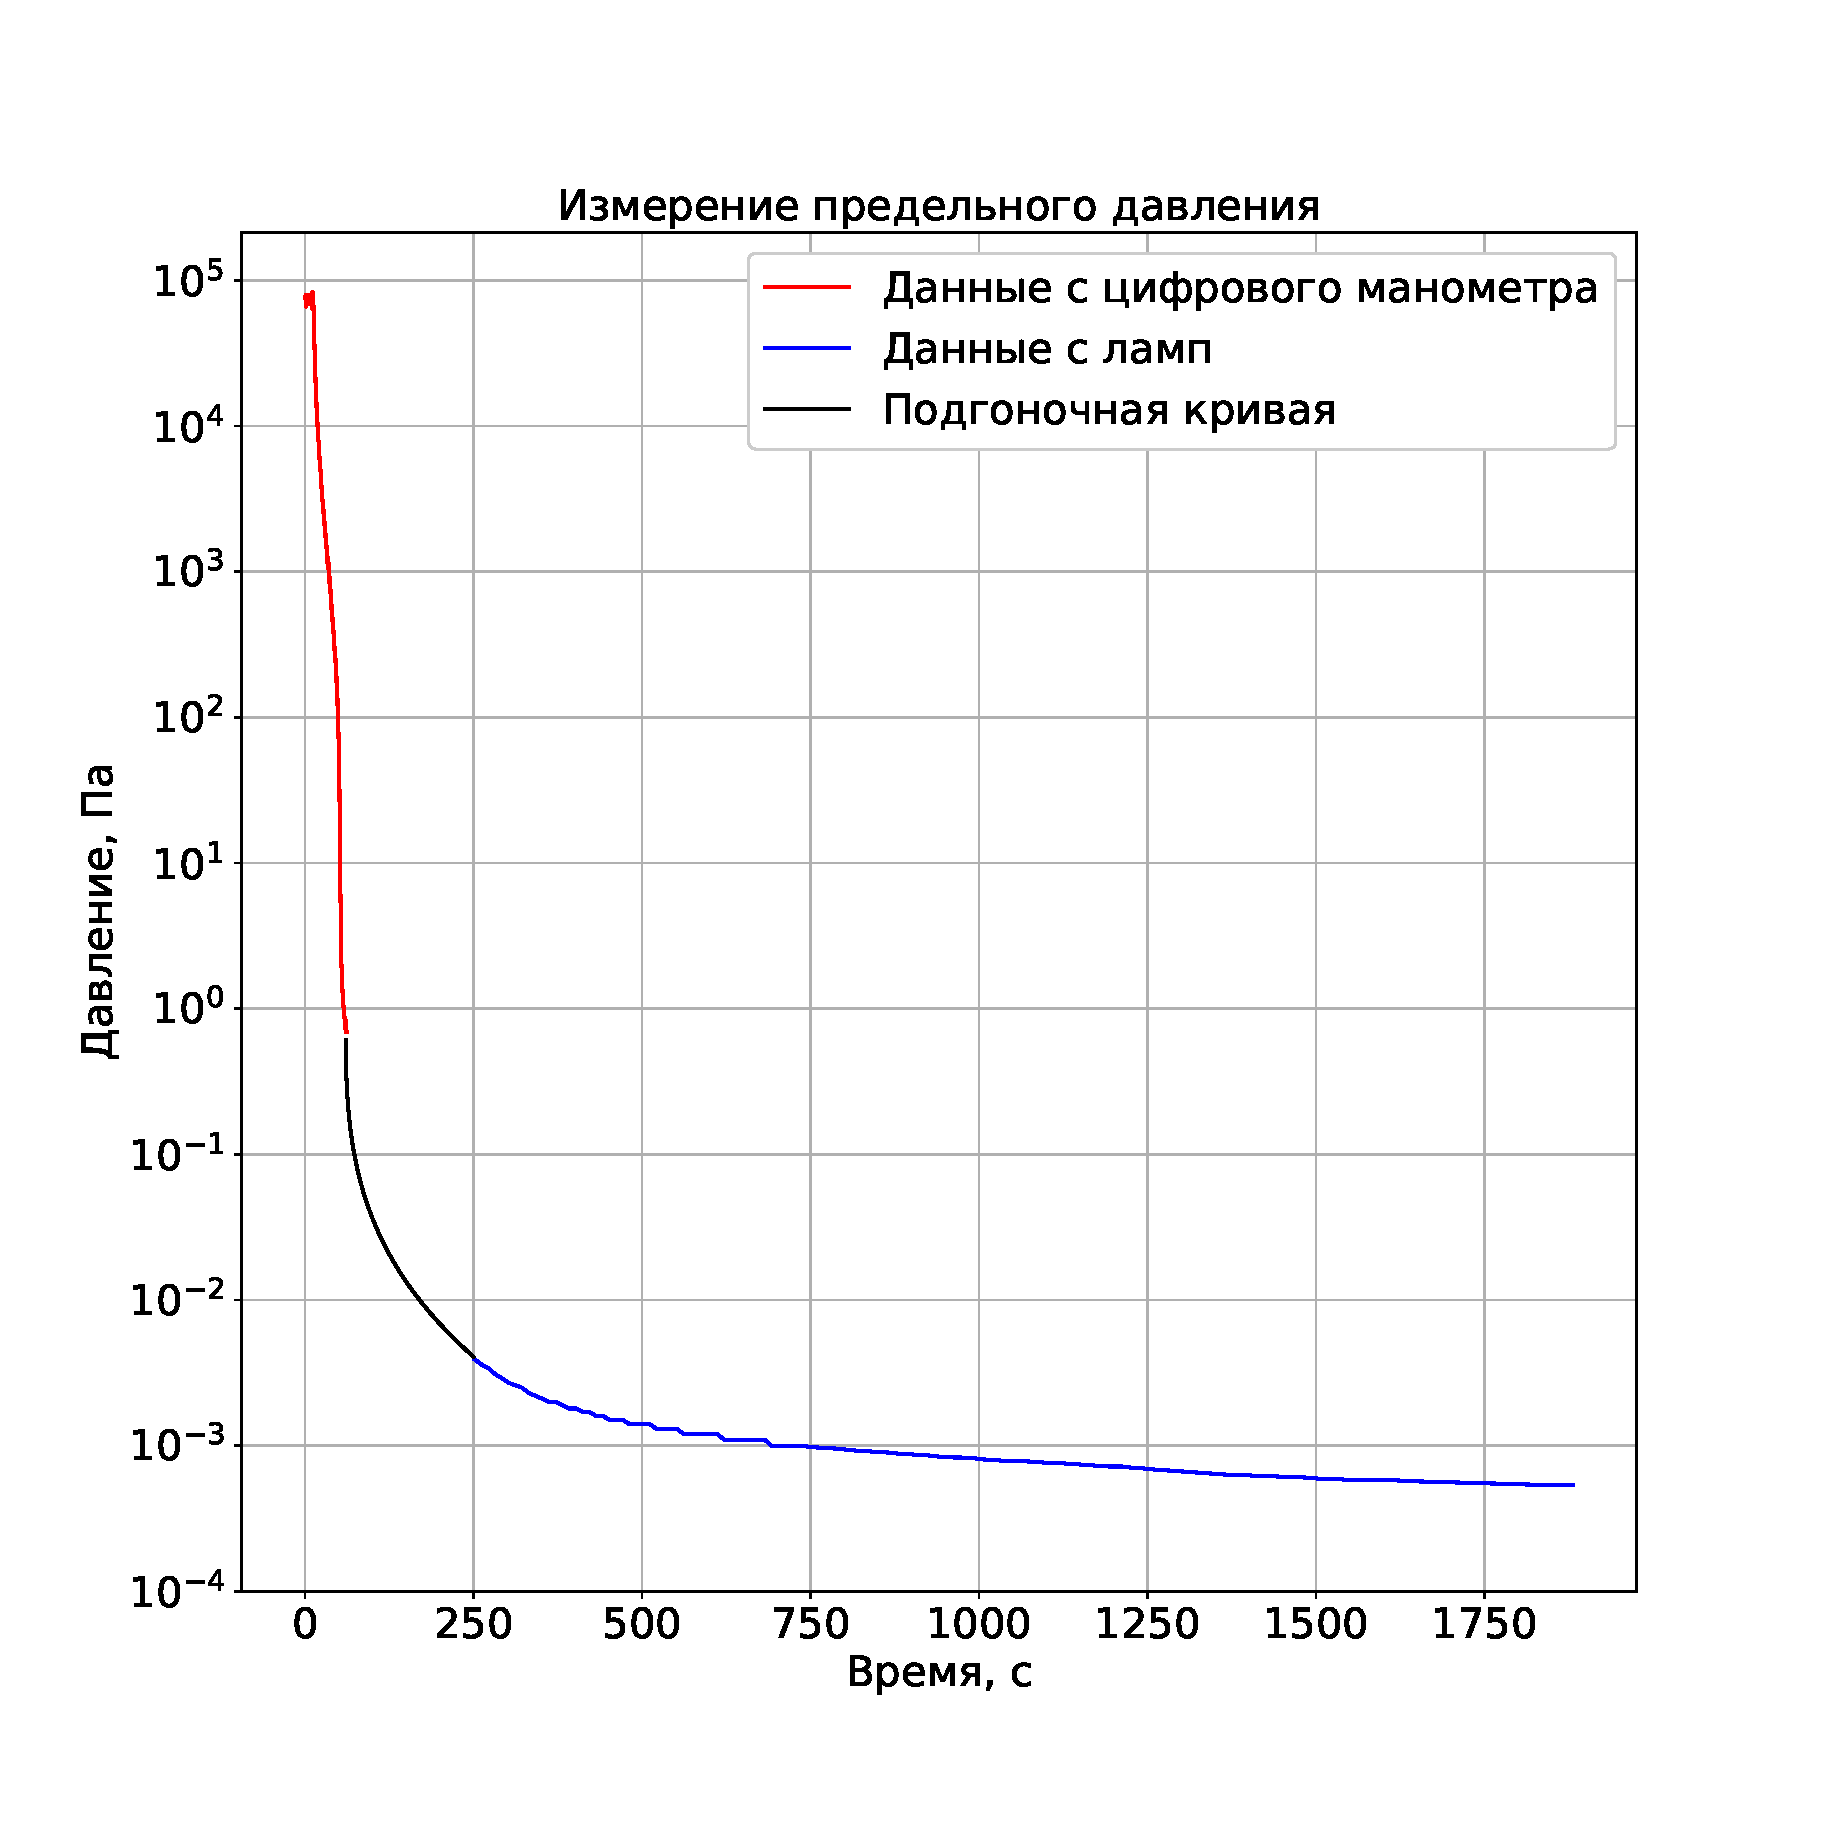
\includegraphics[width=.75\linewidth]{Lab1_1.eps}
				\caption{График зависимости давления от времени в камере}
				\label{fig1}
			\end{figure}
			\newline
			
			Как можно видеть, предельное давление этого насоса оказалось порядка $5 \cdot 10 ^ {-4}$ Па.
			\newpage 
			\begin{figure}[h!]
				\centering
				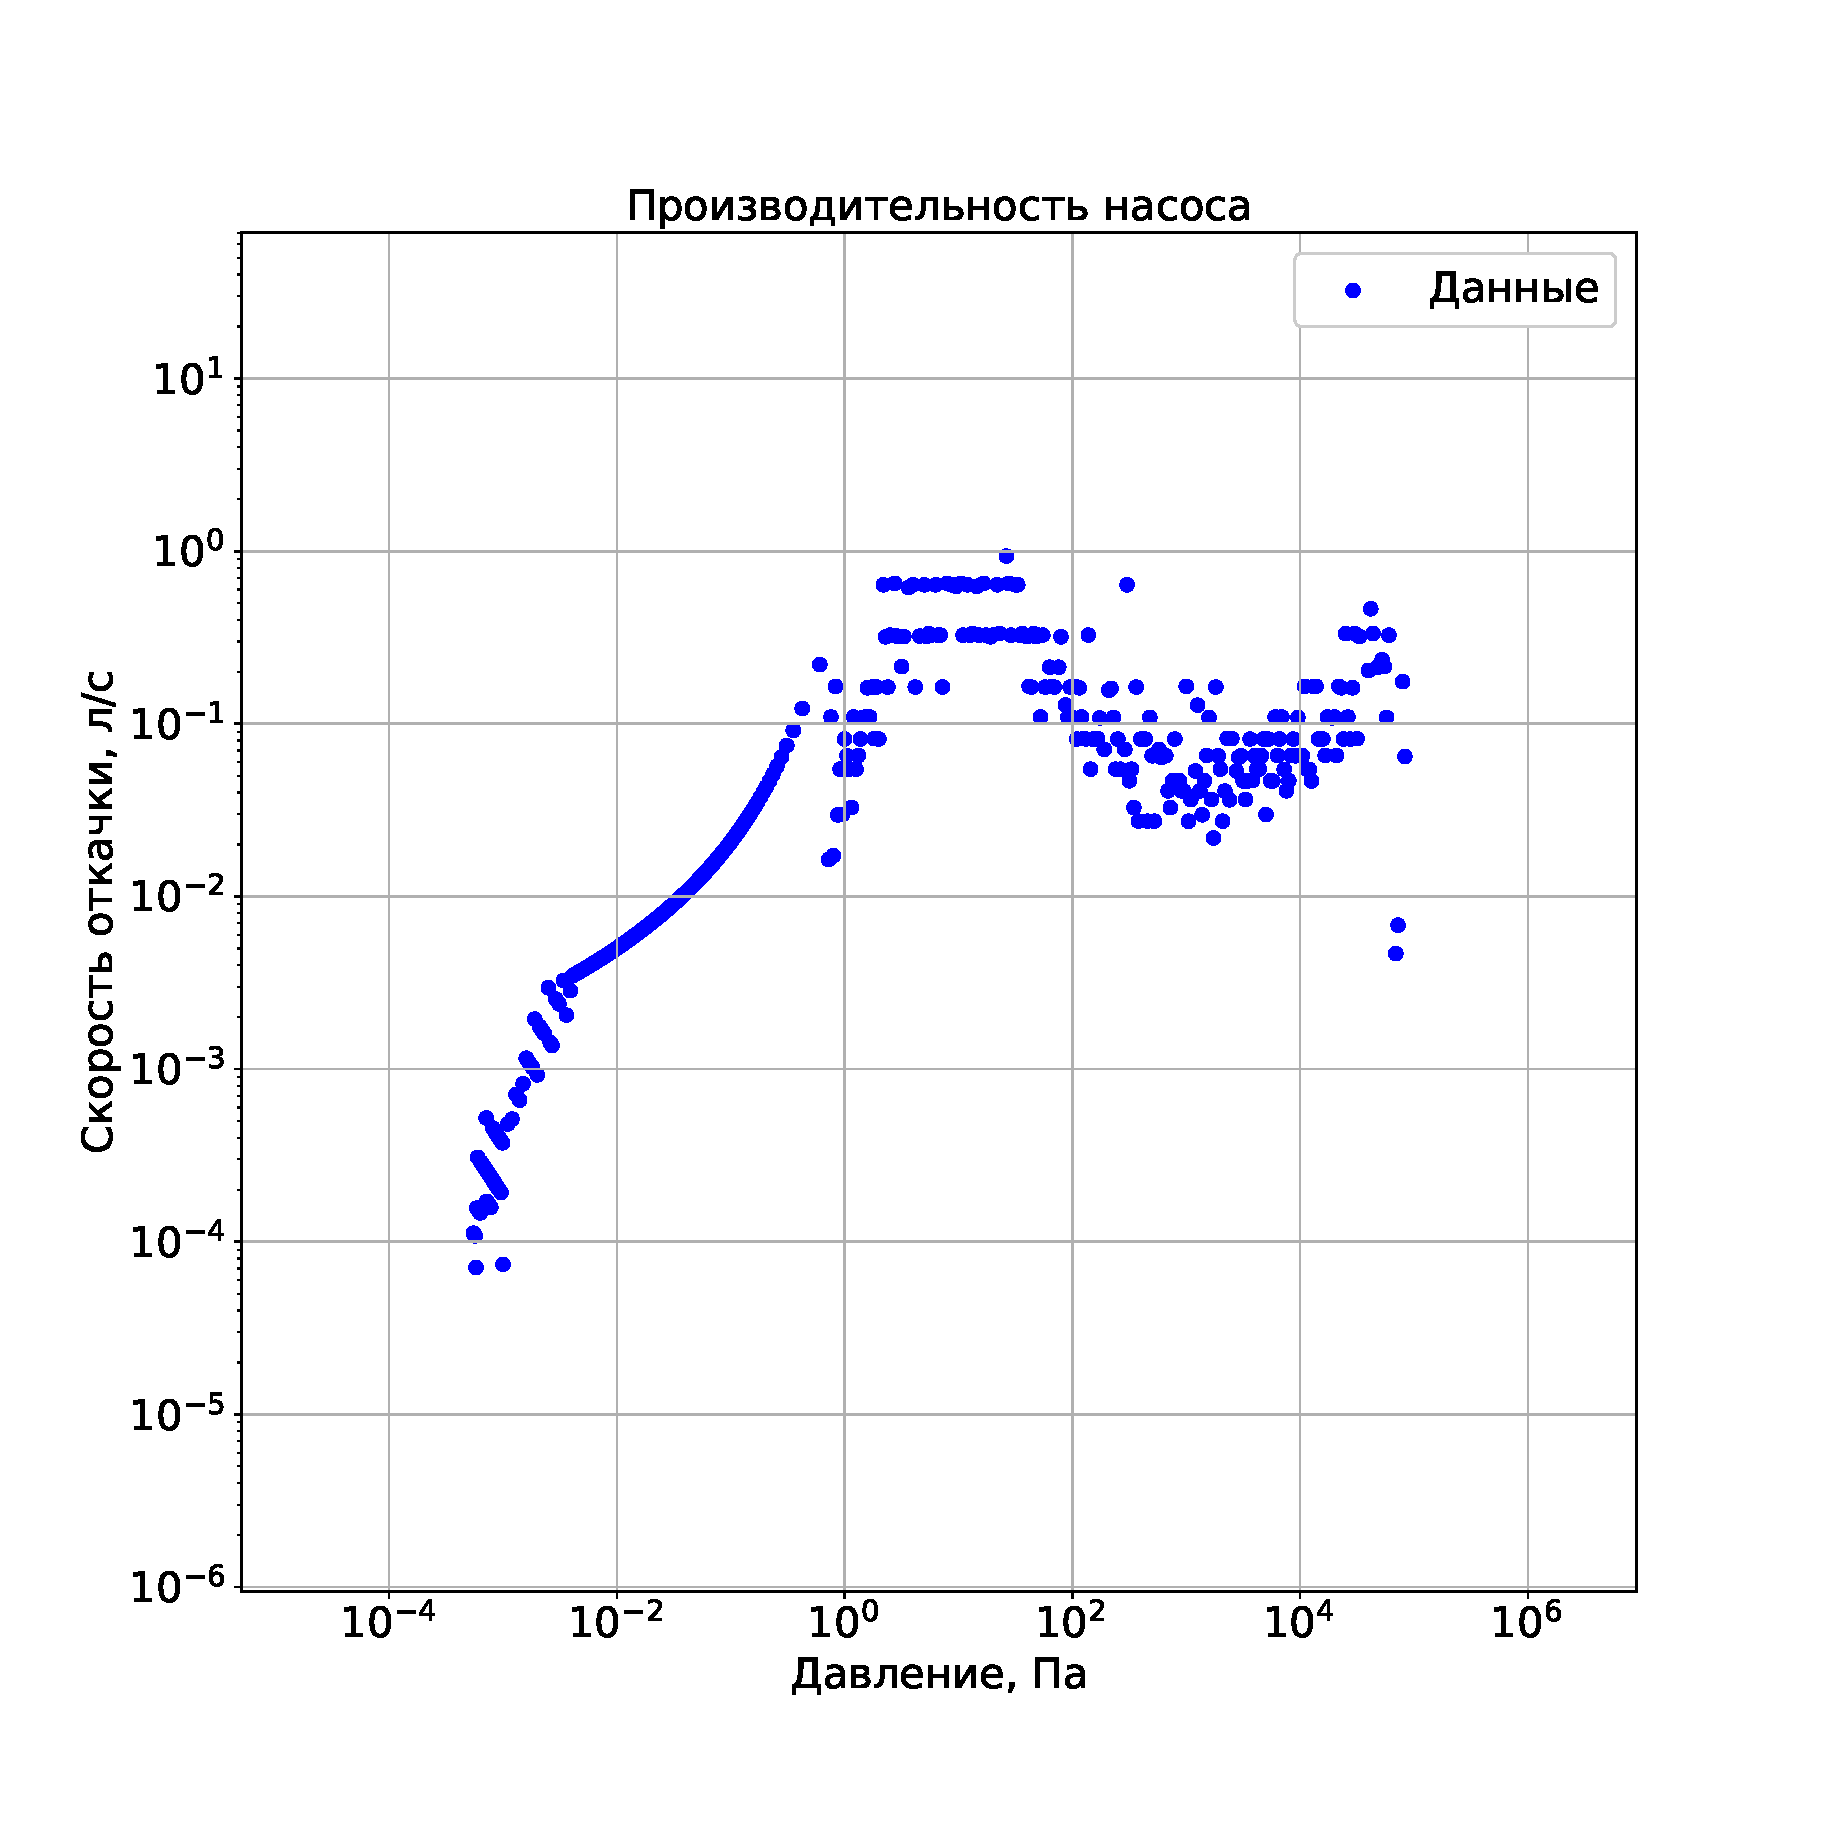
\includegraphics[width=.75\linewidth]{Lab1_2.eps}
				\caption{Производительность насоса}
				\label{fig1}
			\end{figure}
		
			Производительность насоса, как и ожидалось, тем меньше, чем меньше давление в камере. Производительность в ходе эксперимента меняется от $1$ л/c до $7 \cdot 10^{-5}$л/с
	\section{Скорость натекания}
		\subsection{Ход работы}
			К установке в данном эксперименте добавилась камера, соединенная с насосом через сильфонный шланг. Измерить в такой системе предлагалось скорость натекания в камеру. Само натекание проходило достаточно медленно, поэтому было решено закончить измерения через 15-20 минут после эксперимента.
		\subsection{Обработка данных}
			Были построены графики зависимости давления от времени и скорости натекания от давления.
			\begin{figure}[h!]
				\centering
				\includegraphics[width=.55\linewidth]{Screenshot_65.png}
				\caption{Изменение давления вследствие натекания в логарифмических координатах}
				\label{fig1}
			\end{figure}
		
			\begin{figure}[h!]
				\centering
				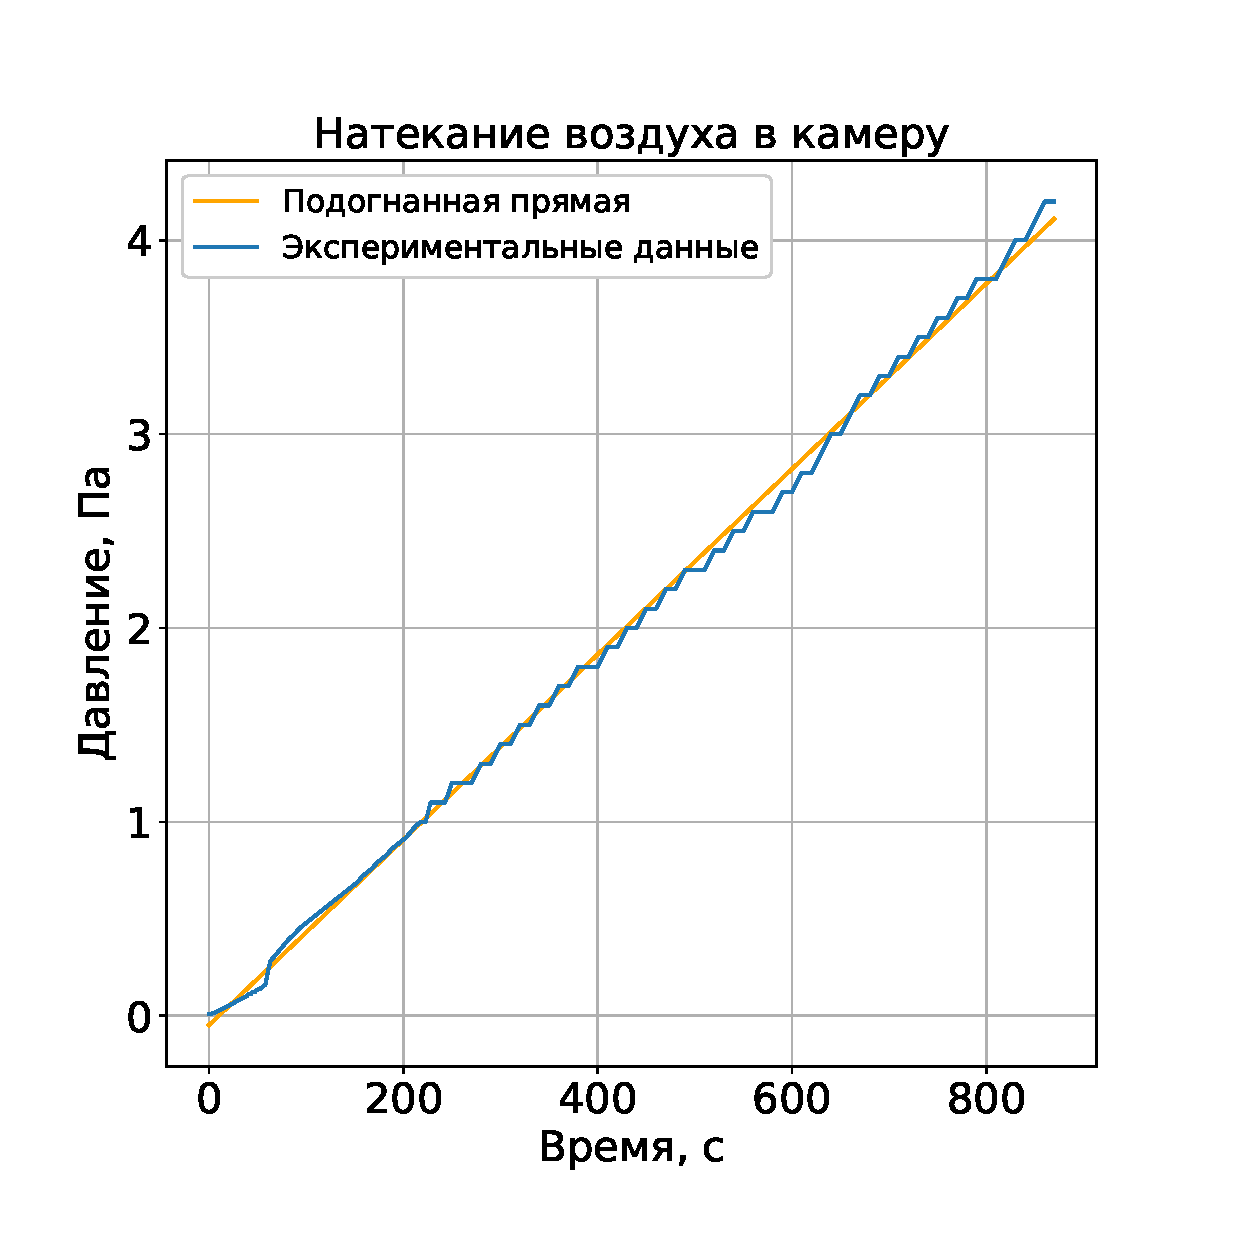
\includegraphics[width=.55\linewidth]{Lab1_3.eps}
				\caption{Изменение давления вследствие натекания}
				\label{fig1}
			\end{figure}
		
			Зависимость давления от времени неплохо описывается прямой. На графике изображено давление сразу после выключения насоса. Начальное давление порядка $10^{-2}$ Па
		
			\begin{figure}[h!]
				\centering
				\includegraphics[width=.55\linewidth]{Screenshot_66.png}
				\caption{График скорости натекания}
				\label{fig1}
			\end{figure}
		
			Далее была найдена скорость натекания, она тоже зависит меняется с увеличением давления. Крайние значения получились следующими: $7 \cdot 10^{-2}$ и $3 \cdot 10 ^ {-4}$ л/с.
	\section{Пропускная способность капилляра}
		\subsection{Ход работы}
			В ходе данного эксперимента мы соединили две камеры капилляром и измеряли его пропускную способность. Измерялось давление в обеих камерах. На камере с насосом использовались ламповые датчики, на второй же камере использовался цифровой датчик, так как давления выходили из диапазона его работы. 
		\subsection{Обработка данных}
			Сначала изобразим графики давления от времени для обеих камер.
			\newpage
			\begin{figure}[h!]
				\centering
				\includegraphics[width=.75\linewidth]{Screenshot_68.png}
				\caption{Давление в камере с насосом}
				\label{fig1}
			\end{figure}
		
			График немного сдвинут по времени из-за того, что манометрические преобразователи ПМИ и ПМТ начинают работу несколько позже из-за своего диапазона измеряемых давлений 
			\begin{figure}[h!]
				\centering
				\includegraphics[width=.75\linewidth]{Screenshot_67.png}
				\caption{Давление во второй камере}
				\label{fig1}
			\end{figure}
			
			В какой-то момент, судя по всему, произошло разъединение контактов манометра, отсюда и небольшие артефакты на графике около нуля.
			
			\newpage
			\begin{figure}[h!]
				\centering
				\includegraphics[width=.75\linewidth]{lab1_9.png}
				\caption{Пропускная способность капилляра}
				\label{fig1}
			\end{figure}
		
			Пропускная способность капилляра, полученная экспериментально, стоит отметить что данные обладают большим количеством шумов. Сравним с теорией
			\begin{figure}[h!]
				\centering
				\includegraphics[width=.75\linewidth]{Screenshot_70.png}
				\caption{Теоретическая зависимость пропускной способности капилляра}
				\label{fig1}
			\end{figure}
		
			Теоретическая зависимость, построенная по формуле $C = \pi r^4 (p_1 + p_2) / (16 \eta l)$ по порядкам лежит близко к полученным данным, однако оценить точность такого метода тяжело из-за шумов на экспериментальных данных.
	\section{Выводы}
		\begin{itemize}
			\item Полученные нами результаты довольно сильно расходятся с паспортными данными для данного откачного поста
			\item Теоретическая зависимость пропускной способности капилляра в целом по порядку близко к экспериментальному значению, но из-за неточности наших данных нельзя сказать большего.
			\item Все соединения были выполнены довольно добротно, так как натекание воздуха происходило весьма медленно
		\end{itemize}
\end{document}